%% ============================================================================
%% main.tex — When sparsity hides the actuator
%% Elsevier elsarticle. Compile: pdflatex main; bibtex main; pdflatex x2.
%% Figures: ../results_scenarios/figures/  |  Bib: ../../articles/references.bib
%% Prose = assembled section drafts. Numbers = 20-seed regen.
%% Floats are placed inline near their first reference (LaTeX floats them to [t]).
%% NOTE: first full draft — run a final numeric pass vs source CSVs before submission.
%% ============================================================================
\documentclass[preprint,3p]{elsarticle}

\usepackage[utf8]{inputenc}
\usepackage[T1]{fontenc}
\usepackage{amsmath,amssymb}
\usepackage{microtype}
\usepackage{graphicx}
\graphicspath{{../results_scenarios/figures/}}
\usepackage{booktabs}
\usepackage[section]{placeins}   % keep floats within their section
\renewcommand{\topfraction}{0.9}
\renewcommand{\bottomfraction}{0.8}
\renewcommand{\textfraction}{0.07}
\renewcommand{\floatpagefraction}{0.75}
\setcounter{totalnumber}{5}
\journal{Computers and Electronics in Agriculture}

\begin{document}

\begin{frontmatter}

\title{When sparsity hides the actuator: a pre-registered economic benchmark of
SINDy-MPC for greenhouse climate control}

\author[a]{Author One}
\author[a]{Author Two}
\affiliation[a]{organization={Affiliation, Department},
  city={City}, country={Country}}

\begin{abstract}
Interpretable data-driven surrogates such as sparse identification of nonlinear
dynamics (SINDy) are attractive for greenhouse model predictive control (MPC)
because they yield explicit, inspectable equations rather than black boxes.
Whether this interpretability comes at an economic cost, however, is rarely tested
under a fair protocol: baselines are often untuned, the metric is a tracking proxy
rather than profit, and---most subtly---the identification recipe is chosen by
open-loop prediction quality. We report a pre-registered, in-silico economic
benchmark of ten controllers on the GreenLight tomato simulator (Rostov-on-Don,
2018--2023 ERA5 weather), using the simulator's own economic performance indicator
(EPI, seasonal profit) as the primary metric and a two-axis Pareto criterion
(EPI versus constraint violations), over 20 seeds with paired non-parametric
statistics. The pre-registered SINDy-MPC recipe, frozen by open-loop metrics
before any closed-loop evaluation, is economically among the weakest interpretable
controllers ($1.18$ vs $4.63~\mathrm{EUR/m^2}$ for a tuned rule-based baseline). A
one-parameter ablation traces the cause: the sparsity threshold zeroes the boiler
term in the temperature equation---the only modelled heating actuator---and
closed-loop EPI collapses from $3.8$ to $1.0~\mathrm{EUR/m^2}$ while the open-loop
rollout error stays flat ($2.25\rightarrow2.39$). The open-loop selection criterion
is thus insensitive to the closed-loop failure it induces. Restoring the term, by a
denser threshold or by DAgger, recovers EPI to parity with the heuristic without
loss of interpretability, and the repaired model coincides with a first-principles
grey-box model. Comparison with additional controllers rules out the obvious
alternative explanations: the true-model oracle over-spends and is not a ceiling, a
normalized PPO improves but does not win, and a black-box NN-MPC is worst---so
neither insufficient fidelity nor interpretability is the bottleneck. The
interpretable surrogate's demonstrable value lies instead in safety and
out-of-distribution guarding, not in economic supremacy. We conclude that parsimony
is not interpretability, that sparsity must be removed from model-selection
objectives when the downstream task is closed-loop control, and that
open-loop-frozen pre-registration can systematically certify a control-catastrophic
model.
\end{abstract}

\begin{keyword}
greenhouse climate control \sep model predictive control \sep
sparse identification of nonlinear dynamics \sep interpretable machine learning \sep
identification for control \sep economic benchmarking
\end{keyword}

\end{frontmatter}

%% ===========================================================================
\section{Introduction}
\label{sec:intro}

Greenhouse horticulture is an energy-intensive industry in which climate control
decisions translate directly into profit: heating, CO\textsubscript{2} enrichment
and supplemental lighting are the dominant variable costs, and they must be balanced
against the revenue from crop growth. Model predictive control (MPC) is a natural
fit, since it optimises a finite-horizon objective subject to the temperature,
humidity and CO\textsubscript{2} constraints that define a productive climate
\citep{vanhenten1994thesis,mayne2000constrained,lin2021greenhousempc}. MPC, however,
needs a model, and first-principles greenhouse models are laborious to build and
calibrate. This motivates data-driven surrogates, and in particular sparse
identification of nonlinear dynamics (SINDy), which recovers explicit governing
equations as a sparse combination of candidate terms
\citep{brunton2016sindy,brunton2016sindyc,kaiser2018sindympc}. Unlike neural
surrogates, a SINDy model is a glass box: its equations can be read, sign-checked
against physics, and embedded analytically in an MPC solver. For a grower or a
certifying body, this interpretability is not a luxury but a practical requirement
for trust and debugging.

The central question is whether interpretability costs performance: whether an
interpretable SINDy-MPC is Pareto-competitive with black-box alternatives, or pays a
measurable ``price of interpretability''. A fair answer is impeded by three
systematic flaws in the comparison procedure itself, common in the
greenhouse-control and learned-control literatures. Learned controllers are often
compared against an under-tuned rule-based baseline, whereas a well-tuned agronomic
heuristic is a strong competitor; setpoint-tracking error is reported in place of
economic profit, although the two are not monotonically related; and, least
obviously, the surrogate's hyper-parameters are chosen by open-loop prediction
accuracy, on the tacit assumption that a more accurate model yields better control.
This last assumption is exactly what identification-for-control has warned against
for three decades \citep{gevers1993,vandenhof1995closedloop}, and what objective
mismatch has re-established for learned dynamics
\citep{lambert2020objective,jacobiandmd2022}.

We address all three by running a pre-registered, in-silico economic benchmark. The
primary metric is the simulator's own economic performance indicator (EPI)---seasonal
profit read directly from the reward model, not a proxy---and, because EPI does not
penalise constraint violations, the primary comparison is a two-axis Pareto criterion
(EPI versus violations). Baselines include a tuned rule-based heuristic and fairly
implemented reinforcement-learning controllers under an equal hyper-parameter budget.
The identification recipe is frozen by open-loop and transparency criteria
\emph{before} any closed-loop evaluation, following pre-registration practice
\citep{pineau2021repro}, so that recipe selection cannot contaminate the honest
comparison. We evaluate ten controllers over 20 seeds with paired non-parametric
statistics \citep{wilcoxon1945,holm1979,efron1994bootstrap}.

The pre-registered hypothesis---that SINDy-MPC is non-dominated at a low price of
interpretability---is not confirmed. The value of the benchmark, however, lies not
in the negative result but in the mechanism it exposes: comparison with additional
controllers isolates the cause of the pre-registered interpretable controller's
underperformance, and this cause is specific and transferable.

The main methodological result is an identified mechanism. The STLSQ sparsity
threshold removes the control-critical boiler actuator term from the model, and
closed-loop EPI follows the presence of that term, whereas the open-loop prediction
error is almost insensitive to its disappearance. As a consequence, a
recipe-selection procedure frozen by open-loop criteria to guard against circular
inference systematically certifies a control-catastrophic model, which is the
pre-registration trap. These findings rest on an honest economic benchmark on a
validated agronomic simulator, in which EPI is verified term-for-term against the
simulator's reward, the rule-based baseline is tuned, the hyper-parameter budget is
equal across methods, and the conclusions are supported by paired statistics over
twenty seeds---something earlier RL-only greenhouse comparisons lacked
\citep{vanlaatum2025greenlightgym}. Finally, the study reconsiders the value of
interpretability itself: it lies in a model's transparency, in safety, and in the
ability to flag out-of-distribution operation, rather than in economic supremacy, and
parsimony of description should not be conflated with interpretability.

%% ===========================================================================
\section{Related work}
\label{sec:related}

Optimal and predictive control of greenhouse climate spans van Henten's
optimal-control formulation of the coupled climate--crop system
\citep{vanhenten1994thesis,vanhenten2009timescale}, modern MPC
\citep{lin2021greenhousempc,chenyou2020ddrmpc}, and stochastic optimal control under
weather uncertainty \citep{vanmourik2023stochastic}. Reinforcement learning (RL) has
been compared against MPC with mixed economic outcomes: RL can raise production but
often at worse profitability
\citep{morcego2023rlvsmpc,mallick2024rlmpc,adaptiverobust2025greenhouse}. The
simulator used here is GreenLight \citep{katzin2020greenlight,katzin2021led}, wrapped
by GreenLight-Gym \citep{vanlaatum2025greenlightgym}. That benchmark, however, is an
RL \emph{environment}: it provides a fast differentiable simulator and benchmarks RL
algorithms, but does not perform an honest economic comparison of controllers against
a tuned rule-based baseline, nor does it consider interpretable sparse-identification
surrogates or the open-loop/closed-loop selection question. The present work occupies
that gap.

SINDy recovers parsimonious governing equations by sparse regression over a candidate
library \citep{brunton2016sindy}, extends to actuated systems \citep{brunton2016sindyc},
and combines naturally with MPC in the low-data limit \citep{kaiser2018sindympc}.
Robustness has been improved by ensembling \citep{fasel2022ensemble}, relaxed and
constrained optimisation \citep{champion2020sr3}, and mature tooling
\citep{desilva2020pysindy,kaptanoglu2022pysindy}. The sequentially-thresholded
least-squares (STLSQ) core, however, is sensitive to its sparsity threshold: too
large a threshold removes physically important small-coefficient terms, degrading the
dynamics \citep{cortiella2021sparse,mangan2017modelselection}, a problem that recent
optimisers explicitly target \citep{balanceguided2026}. Prior work treats this as an
\emph{identification} pathology and proposes better \emph{optimisers}; here its
consequence is instead diagnosed inside an economic MPC loop, with an established
causal link to profit, showing that a standard open-loop selection protocol walks
straight into it.

That open-loop prediction accuracy is a poor proxy for closed-loop control is a
foundational message of identification-for-control: the loop, not the fit, must
arbitrate model quality \citep{gevers1993,hjalmarsson1994closing,%
vandenhof1995closedloop,hjalmarsson2005experiment}. The same phenomenon was sharpened
for learned dynamics as objective mismatch---one-step likelihood is not correlated
with control performance \citep{lambert2020objective,wei2023unified}---with related
remedies in value-aware and control-oriented model learning
\citep{farahmand2017value,controlorientedsurvey2025}. The contribution here is neither
the general principle nor a new remedy, but a concrete, interpretable, and causally
verified instance of it: because the surrogate is a glass box, the failure is legible
term-by-term (a single removed actuator) rather than diagnosed by re-weighting a
black-box model. To restore the term we use dataset aggregation (DAgger)
\citep{ross2011dagger}, an established bridge between an MPC expert and a learned model
\citep{sun2017deeply,tagliabue2021guided,espin2024deepmpc}.

%% ===========================================================================
\section{Methods}
\label{sec:methods}

\textbf{Primary metric.}~All controllers are scored by the simulator's own economics
rather than a proxy. At each step the GreenLight reward model returns a profit
$\pi_k = g_k - c_k$, where the gain $g_k = (x^{\mathrm{fruit}}_k -
x^{\mathrm{fruit}}_{k-1})\,\tfrac{10^{-6}}{\mathrm{dmfm}}\,p_{\mathrm{fruit}}$ is the
revenue from fruit dry-matter growth (converted to fresh weight through the
dry-to-fresh ratio $\mathrm{dmfm}=0.065$ and priced at
$p_{\mathrm{fruit}}=1.6~\mathrm{EUR/kg}$), and the variable cost $c_k$ sums heating,
lighting and CO\textsubscript{2} dosing priced at $0.09~\mathrm{EUR/kWh}$,
$0.30~\mathrm{EUR/kWh}$ and $0.30~\mathrm{EUR/kg}$. The seasonal indicator is
$\mathrm{EPI}=\sum_k \pi_k$ $[\mathrm{EUR/m^2}]$. We verified that the per-step
economics used by every controller (and by the oracle, below) are identical
term-for-term to the simulator's reward, so EPI is the ground-truth objective and not
an approximation. Because EPI omits constraint penalties and a controller can raise it
by spending more time outside the productive corridors
(CO\textsubscript{2}$\in[300,1600]$~ppm, $T\in[15,34]~^\circ$C, RH$\in[50,85]\%$), the
primary comparison is a two-axis Pareto criterion---EPI versus the seasonal count of
violation steps---reported with a non-dominated frontier (Fig.~\ref{fig:pareto}). As a
secondary, dimensionally consistent severity scalar we report \texttt{scaled\_pen},
the violation area per constraint normalised by the simulator's own scaling. We do not
combine EPI and violations into a single ``EUR-penalised EPI'', since the simulator
does not price violations.

\textbf{Simulator, location and data.}~Experiments use the GreenLight tomato model
\citep{katzin2020greenlight} through the GreenLight-Gym interface
\citep{vanlaatum2025greenlightgym}. The location is Rostov-on-Don ($47.24^\circ$N,
$39.71^\circ$E); real weather for 2018--2023 is from ERA5/ERA5-Land via Open-Meteo,
with derived sky and soil terms. A season is 60 days starting 1 March, at a 15-minute
control period. We use a leakage-free year split: training on 2018--2019,
in-distribution test on 2020, and 2021--2023 held out as out-of-distribution (OOD).
Identification data are collected by the rule-based controller augmented with a
pseudo-random binary excitation signal (PRBS, amplitude $0.3$) on the actuators, with
the regression condition number monitored.

\textbf{Controllers.}~We compare ten controllers spanning five families
(Table~\ref{tab:controllers}): a tuned rule-based agronomic heuristic (the lower
reference and the DAgger expert); the proposed SINDy-MPC in four variants---the
pre-registered confirmatory recipe, a boiler-preserving dense recipe, and
DAgger-repaired versions of each; a reduced first-principles grey-box MPC that reuses
the same solver; a neural-network MPC (NN-MPC, $64{\times}64$ surrogate); two
reinforcement-learning policies, PPO \citep{schulman2017ppo} and SAC
\citep{haarnoja2018sac}, via Stable-Baselines3 \citep{raffin2021sb3}; and an oracle
MPC that plans over the true simulator dynamics. All learned controllers receive an
equal hyper-parameter budget (16 trials). RL is trained for $2\times10^5$ environment
steps with observation and reward normalisation (VecNormalize), whose omission we
found to distort the RL result badly.

\begin{table*}[t]
\centering
\caption{Controllers and the role of each. The set is chosen to rule out, in turn, the
alternative explanations for the pre-registered interpretable method's underperformance.}
\label{tab:controllers}
\small
\begin{tabular}{@{}p{3.0cm}p{2.4cm}p{5.2cm}p{4.0cm}@{}}
\toprule
Controller & Class & Alternative explanation tested & Answer from data \\
\midrule
Rule-based & tuned heuristic & existence of a strong simple target (also DAgger expert) & yes --- EPI 4.63, the bar \\
Grey-box MPC & reduced physics & weakness of the MPC/library itself & no --- 3.79 works; the threshold is the cause \\
SINDy-MPC (confirmatory) & proposed, pre-reg. & the method under test & fails: 1.18 (boiler dropped) \\
SINDy-MPC (dense/+DAgger) & proposed, repaired & fixability without losing interpretability & yes --- 3.8--5.2, still glass-box \\
Oracle (3\,h CEM) & true-model MPC & insufficient model fidelity & no --- 1.99, over-spends \\
NN-MPC & black-box surrogate & a black-box advantage & no --- $-5.09$, worst \\
PPO / SAC & black-box RL & interpretability as the bottleneck & no --- both below the heuristic \\
\bottomrule
\end{tabular}
\end{table*}

\textbf{Pipeline and pre-registration.}~The proposed method has four stages. The
rule-based controller with a superimposed PRBS signal first collects data; sparse
regression then identifies an interpretable discrete one-step map
$x_{k+1}=\Xi\,\Theta(x_k,u_k,d_k)$ of degree~1, low enough for analytic MPC embedding;
the resulting surrogate is embedded in a CasADi/do-mpc solver that optimises an
EPI-aligned objective under the climate constraints on a finite horizon; and, where
needed, online adaptation (DAgger or EKF-SINDy) is added with an OOD monitor and a
safe fallback. The identification recipe
(denoising, optimiser and library) is not fixed a priori: it is selected in an
ablation (E2) and then frozen by open-loop identification metrics (multi-step rollout
stability, MPC-embeddability, transparency) \emph{before} and \emph{independently of}
any closed-loop EPI on the held-out test season; this pre-registration guards against
circular inference. The frozen confirmatory recipe uses the \texttt{physics\_no\_cross}
library, degree~1, and an ensemble optimiser; a closed-loop-selected exploratory
recipe is recorded separately and reported only as post-hoc sensitivity. The identical
frozen recipe is loaded by every downstream experiment through a single source of truth.

\textbf{Gates and statistics.}~A model is admitted only if it passes a transparency
gate (glass-box equations, a threshold fraction of passed physical sign/dimension
checks, bootstrap structural stability of the active-term set) and an
MPC-embeddability gate. Both gates are deliberately open-loop; their consequences are
examined below. The source of variance is the re-collection of training data per
seed: each seed re-collects the identification dataset and re-fits the surrogate, so
per-seed models genuinely differ. We use 20 seeds for all controllers; SAC converged
on only 10 of 20 and is reported on those. Pairwise comparisons use the Wilcoxon
signed-rank test paired by seed \citep{wilcoxon1945} with Holm correction
\citep{holm1979}, reporting Cohen's $d$ and bootstrap 95\% confidence intervals
\citep{efron1994bootstrap,demsar2006}.

\textbf{The oracle.}~The oracle is a receding-horizon cross-entropy-method (CEM)
controller that plans directly over the true simulator integrator (48 sampled action
sequences, a 3-hour horizon, two refinement iterations, warm-started from the
rule-based action), with the same economic objective as the MPC. The gap between it
and a surrogate-based MPC isolates the effect of model fidelity. It is not an upper
bound on seasonal EPI: a short receding horizon greedily maximises short-horizon
profit, and the sampling optimiser degrades at longer horizons, so it is treated as a
fidelity control rather than a ceiling.

%% ===========================================================================
\section{Results}
\label{sec:results}

The ten controllers are chosen to isolate the cause of the interpretable controller's
underperformance by ruling out the obvious alternative explanations (a weak MPC,
insufficient model fidelity, a black-box advantage). Verdicts on the pre-registered
hypotheses are summarised in Table~\ref{tab:scorecard}.

\begin{table}[t]
\centering
\caption{Hypothesis scorecard (pre-registered H1--H4, 20-seed verdicts).}
\label{tab:scorecard}
\small
\begin{tabular}{@{}p{2.0cm}p{2.0cm}p{3.2cm}@{}}
\toprule
Hypothesis & Verdict & Evidence \\
\midrule
Central & not confirmed & conf+DAgger ties RB ($p{=}0.26$); confirmatory sig.\ worse \\
H1 (gap-to-oracle) & not met & oracle 1.99 $<$ RB/PPO/grey-box \\
H2 (rollout stability) & met, but insufficient & RMSE stable yet closed-loop collapses \\
H3 (transparency) & partial & beats NN-MPC; confirmatory $<$ grey-box \\
H4a (adaptation) & not supported & DAgger $+0.39$, $p{=}0.088$; EKF worse \\
H4b (OOD guard) & supported & guard $-50\%$ viol, $p{\approx}10^{-24}$ \\
H4c (no exploitation) & partial & confirmatory over-violates; guard mitigates \\
\bottomrule
\end{tabular}
\end{table}

The E2 ablation over denoising, optimiser, library and degree (42 recipes) selected,
by open-loop rollout stability and the transparency and embeddability gates, a recipe
with the \texttt{physics\_no\_cross} library, degree~1, and an ensemble optimiser as
the confirmatory recipe, frozen before any closed-loop evaluation. Multi-step rollout
divergence is negligible for this recipe (diverged-trajectory fraction $\approx 0$ for
budgets $\ge 3$ days), so it passes the open-loop bar that pre-registration relies on.
Hypothesis~\textbf{H2} (a stable-rollout recipe exists) is thus met; but, as shown
below, open-loop stability is necessary and not sufficient.

Table~\ref{tab:e3main} reports the 20-seed closed-loop EPI, violations and severity
for all ten controllers, with paired significance against the rule-based baseline;
Fig.~\ref{fig:pareto} shows the EPI--violation Pareto plane. Only the DAgger-repaired
SINDy-MPC reaches the top: $5.23\pm2.40~\mathrm{EUR/m^2}$, statistically
indistinguishable from the rule-based $4.63$ ($\Delta=+0.59$, $p_{\mathrm{Holm}}=0.26$).
Every other controller is significantly worse than the tuned heuristic: the grey-box
MPC ($3.79$, $p_{\mathrm{Holm}}=0.017$), PPO ($3.36$, $p_{\mathrm{Holm}}=0.001$), the
pre-registered confirmatory SINDy-MPC ($1.18$, $p_{\mathrm{Holm}}=0.009$), SAC
($-2.41$) and NN-MPC ($-5.09$, $p_{\mathrm{Holm}}\approx2\times10^{-5}$). The
non-dominated frontier comprises the DAgger-repaired SINDy-MPC, the rule-based
heuristic, PPO, and---as a degenerate minimum-violation corner with negative EPI---SAC.
On the severity axis the DAgger SINDy-MPC accrues even a lower total violation severity
than the rule-based controller ($426$ vs $485$) despite more violation steps; both axes
are therefore reported together. The central pre-registered hypothesis is thus not
confirmed, and the only interpretable controller that matches the heuristic achieves
this through a repair whose mechanism is examined next.

\begin{table*}[t]
\centering
\caption{E3 closed-loop economic benchmark (20 seeds), by decreasing EPI. $\Delta$EPI
and $p_{\mathrm{Holm}}$ are the paired Wilcoxon test vs Rule-based with Holm correction.
Frontier $=$ non-dominated in (EPI $\uparrow$, violation-steps $\downarrow$).}
\label{tab:e3main}
\small
\begin{tabular}{@{}lrrrrrrrc@{}}
\toprule
Controller & EPI & Viol. & scaled & $T$-corr & $n$ & $\Delta$EPI & $p_{\mathrm{Holm}}$ & Front. \\
 & (EUR/m$^2$) & steps & pen & \% & & vs RB & & \\
\midrule
SINDy-MPC (conf+DAgger) & $5.23\pm2.40$ & 4302 & 426 & 62 & 20 & $+0.59$ & 0.26 (ns) & $\bullet$ \\
Rule-based & $4.63\pm0.00$ & 2458 & 485 & 95 & 20 & --- & --- & $\bullet$ \\
SINDy-MPC (dense) & $3.81\pm1.27$ & 6073 & 1206 & 65 & 20 & $-0.82$ & 0.017 & \\
Grey-box MPC & $3.79\pm1.27$ & 6083 & 1209 & 65 & 20 & $-0.85$ & 0.017 & \\
PPO & $3.36\pm1.59$ & 1842 & 392 & 84 & 20 & $-1.28$ & 0.001 & $\bullet$ \\
SINDy-MPC (dense+DAgger) & $3.23\pm2.21$ & 4467 & 624 & 66 & 20 & $-1.40$ & 0.031 & \\
Oracle (3\,h CEM) & $1.99\pm0.68$ & 2816 & 379 & 72 & 20 & $-2.65$ & 2e{-}5 & \\
SINDy-MPC (confirmatory) & $1.18\pm4.33$ & 5357 & 793 & 50 & 20 & $-3.46$ & 0.009 & \\
SAC & $-2.41\pm1.24$ & 1683 & 179 & 82 & 10 & $-7.04$ & 0.010 & $\bullet$ \\
NN-MPC & $-5.09\pm3.11$ & 4368 & 767 & 70 & 20 & $-9.72$ & 2e{-}5 & \\
\bottomrule
\end{tabular}
\end{table*}

\begin{figure}[htbp]
\centering

\includegraphics[width=\linewidth]{e3_pareto_annotated.png}
\caption{E3 Pareto plane (EPI $\times$ violations, 20 seeds). The non-dominated
frontier (red) is rule-based, SINDy-MPC(conf+DAgger), PPO, and SAC (degenerate
minimum-violation corner). The repaired dense SINDy-MPC coincides with the grey-box
model: parsimony is not interpretability.}
\label{fig:pareto}
\end{figure}

\textbf{Mechanism: sparsity hides the actuator.}~The pre-registered confirmatory recipe
is the weakest of the interpretable controllers ($1.18\pm4.33$, against $4.63$ for the
rule-based baseline and $3.79$ for the grey-box MPC that shares its solver and feature
library). Yet the recipe was not selected for weak closed-loop control: it was frozen,
before any closed-loop evaluation, as the most parsimonious model passing the open-loop
and transparency gates. The recipe that pre-registration certified as
identification-optimal is thus the recipe that fails in the loop.

We isolate the cause with a one-parameter ablation. Holding the feature library
(\texttt{physics\_no\_cross}, degree~1) and the MPC fixed, the STLSQ sparsity threshold
$\lambda$ is swept over $[10^{-6},10^{-1}]$; at each value, over 20 seeds, we record the
number of surviving coefficients, the signed boiler coefficient in the temperature
equation $\Xi_{u_{\mathrm{Boil}}\rightarrow T_{\mathrm{in}}}$ (the greenhouse's only
modelled active heating actuator), the \emph{open-loop} rollout-RMSE of $T_{\mathrm{in}}$
on the deployment season, and the \emph{closed-loop} EPI (Fig.~\ref{fig:lambda},
Table~\ref{tab:lambda}).

\begin{figure}[htbp]
\centering

\includegraphics[width=\linewidth]{e3_lambda_sweep_ablation.png}
\caption{Sweeping the STLSQ sparsity threshold $\lambda$: closed-loop EPI (blue)
collapses as the boiler coefficient $u_{\mathrm{Boil}}\!\to\!T_{\mathrm{in}}$ (green) is
thresholded to zero, while the open-loop rollout-RMSE (red) stays flat. Open-loop model
selection is insensitive to the closed-loop failure.}
\label{fig:lambda}
\end{figure}

\begin{table}[t]
\centering
\caption{Sparsity-threshold sweep ($\lambda$) of the \texttt{physics\_no\_cross}
degree-1 surrogate, 20 seeds. The boiler coefficient and closed-loop EPI collapse
around $\lambda\!\approx\!0.05$ while open-loop rollout-RMSE stays flat.}
\label{tab:lambda}
\small
\begin{tabular}{@{}rrrrr@{}}
\toprule
$\lambda$ & nonzero & $\Xi_{u_{\mathrm{Boil}}\to T_{\mathrm{in}}}$ & rollout-RMSE & EPI \\
\midrule
$10^{-6}$ & 54.0 & 0.036 & 2.25 & 3.79 \\
$10^{-3}$ & 49.9 & 0.036 & 2.25 & 3.81 \\
0.01 & 41.8 & 0.036 & 2.27 & 4.00 \\
0.02 & 38.4 & 0.035 & 2.27 & 4.67 \\
0.03 & 34.8 & 0.032 & 2.28 & 3.49 \\
0.04 & 30.8 & 0.021 & 2.37 & 1.14 \\
0.05 & 27.7 & 0.006 & 2.38 & 0.99 \\
0.10 & 20.3 & 0.000 & 2.39 & 2.49 \\
\bottomrule
\end{tabular}
\end{table}

Two quantities move in opposite directions. As $\lambda$ increases from $10^{-6}$ to
$0.1$ the model becomes more parsimonious (surviving terms $54\rightarrow20$) and the
boiler coefficient decays and vanishes:
$\Xi_{u_{\mathrm{Boil}}\rightarrow T_{\mathrm{in}}}\approx0.035$ for $\lambda\le0.02$,
$0.032$ at $\lambda=0.03$, $0.006$ at $\lambda=0.05$, and exactly $0$ at $\lambda=0.1$.
Closed-loop EPI tracks this collapse---from a peak of $4.67$ at $\lambda=0.02$ to $0.99$
at $\lambda=0.05$, exactly where the boiler term is thresholded out. Once the surrogate
contains no heating actuator, the MPC cannot plan heating, and in a heating-dominated
spring the loss is severe. The open-loop metric, by contrast, is almost inert:
rollout-RMSE moves only from $2.25$ to $2.39$ (a $6\%$ change) while EPI moves by a
factor of five and the boiler term disappears. The pre-registered open-loop criterion
is therefore insensitive to the closed-loop failure it causes. This is a concrete,
physically legible instance of the mismatch between predictive accuracy and control
performance \citep{lambert2020objective,jacobiandmd2022}, and a sparse-identification
realisation of the identification-for-control principle that the closed loop must
arbitrate model quality \citep{gevers1993,vandenhof1995closedloop}.

If removal of the boiler term is the cause, restoring it should recover performance,
and two independent interventions do so (Table~\ref{tab:e3main}). A dense recipe
(\texttt{stlsq}, $\lambda=10^{-3}$) keeps
$\Xi_{u_{\mathrm{Boil}}\rightarrow T_{\mathrm{in}}}\approx0.034$ and lifts EPI from
$1.18$ to $3.81$; DAgger applied to the confirmatory recipe reintroduces the term
through closed-loop data and lifts EPI to $5.23$, indistinguishable from the rule-based
baseline. Across all SINDy-MPC variants, EPI is monotone in the presence of the boiler
coefficient: whenever $\Xi_{u_{\mathrm{Boil}}\rightarrow T_{\mathrm{in}}}\neq0$, it rises
from $\approx1$ to $4$--$5~\mathrm{EUR/m^2}$. The boiler coefficient is a one-dimensional
causal proxy for economic competence.

The dense fix is not a black box: it is the same glass-box map with more non-zero terms,
and the repaired dense SINDy-MPC ($3.81$) coincides with the first-principles grey-box
MPC ($3.79$) to within noise (Fig.~\ref{fig:pareto}). Once over-sparsification is
removed, the interpretable surrogate collapses onto the physical model it was meant to
replace. What sparsity removed was neither accuracy nor transparency but the
controllability conferred by a single small-magnitude actuator term. Two practical
implications follow. Sparsity should not be a model-selection objective when the task is
closed-loop control \citep{farahmand2017value,cortiella2021sparse,balanceguided2026}; and
a transparency gate that certifies a model whose key actuator has been zeroed is
incomplete---a dropped key actuator should itself be a gate failure.

\textbf{Model fidelity does not explain the shortfall.}~If the shortfall were due to an
inaccurate surrogate, an MPC over the true model should win. It does not: the oracle
returns only $1.99\pm0.68~\mathrm{EUR/m^2}$ (Table~\ref{tab:e3main}), below the heuristic,
the DAgger and dense/grey-box models, and PPO. A horizon probe (Fig.~\ref{fig:oracle})
explains why: EPI falls rather than rises with horizon ($+0.26$ at 3~h, $+0.04$ at 12~h,
$-0.51$ at 24~h on a 14-day window where the rule-based controller scores $+0.63$). Fruit
growth and revenue rise toward the heuristic's level as the horizon lengthens, but cost,
chiefly electricity and CO\textsubscript{2}, rises faster, so the oracle attains
comparable production more expensively. This is greedy over-spend from a short receding
horizon, not a fidelity deficit, so the ``gap-to-oracle'' framing (hypothesis
\textbf{H1}) is not a meaningful ceiling here. It is a structural property of
short-horizon economic MPC, not an experimental error: the oracle correctly maximises
the very quantity the simulator rewards, only greedily and over too short a window.

\begin{figure}[htbp]
\centering
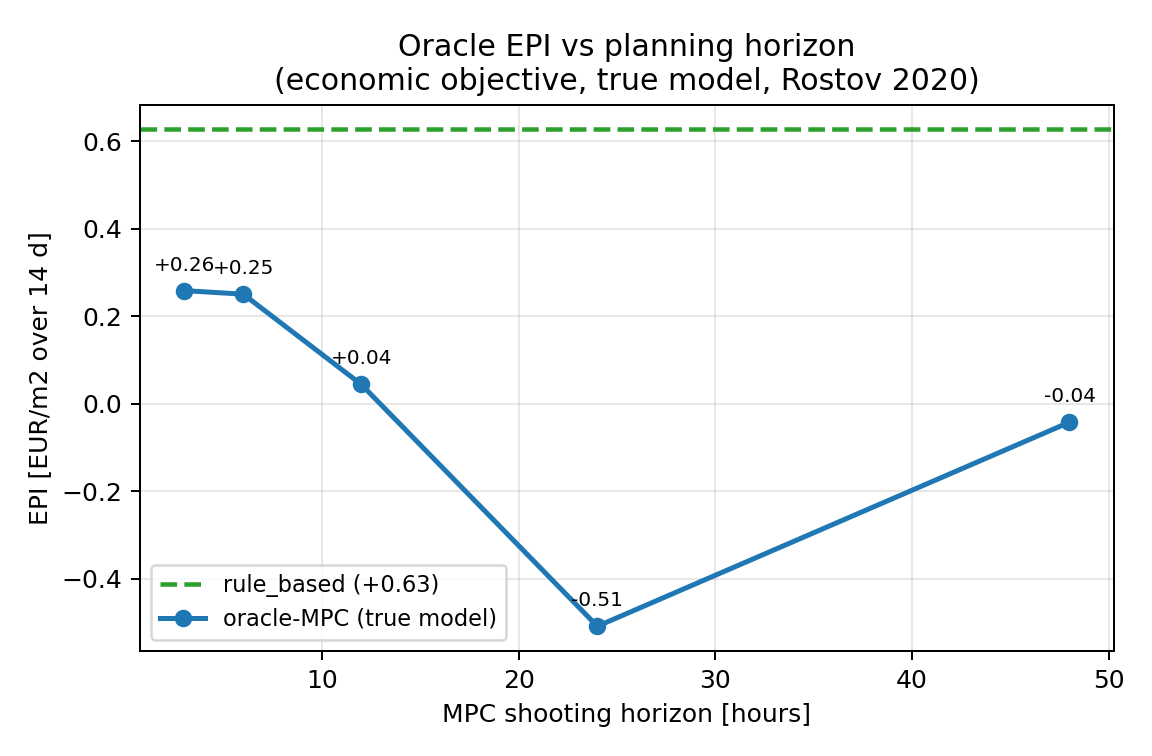
\includegraphics[width=0.82\linewidth]{oracle_horizon_sweep.png}
\caption{The oracle is not a ceiling. EPI of the true-model economic MPC falls as its
planning horizon lengthens and stays below the rule-based heuristic (dashed): a short
receding horizon greedily over-spends.}
\label{fig:oracle}
\end{figure}

\textbf{Interpretability is not the bottleneck.}~A black-box learner does not win either.
RL baselines are sensitive to normalisation: a naive PPO scores $-13~\mathrm{EUR/m^2}$,
whereas standard observation/reward normalisation lifts it to $+3.4$---a reproducibility
lesson rather than a property of RL \citep{henderson2018matters}---yet even the normalised
PPO ($3.36$) remains significantly below the heuristic over 20 seeds, and SAC is unstable,
diverging on 10 of them. The black-box NN-MPC, in turn, is the worst controller in the
study ($-5.09~\mathrm{EUR/m^2}$), beaten by every interpretable SINDy variant.

\textbf{Online adaptation is a null.}~Under spring OOD shifts (2021--2023, same planting
season), the offline surrogate already generalises well---mean EPI $\approx0$, beating the
rule-based controller's $-2.9$ under the same shift---leaving little gap for adaptation.
Over 60 (shift $\times$ seed) pairs, DAgger improves on the static offline model by only
$+0.39~\mathrm{EUR/m^2}$ ($p=0.088$, not significant), and online EKF-SINDy is significantly
worse ($-2.17$, $p<10^{-6}$); an earlier smaller sample ($n=9$) suggesting a significant
DAgger gain does not survive. Hypothesis~\textbf{H4a} is not supported. The failure under
shift is not gradual coefficient drift but a data problem: single-season on-shift data are
intrinsically confounded ($\mathrm{corr}(u_{\mathrm{Vent}},T_{\mathrm{in}})=+0.67$ against
$+0.03$ for multi-year offline data), so a re-fit mislearns the ventilation effect. What
confers OOD robustness is structure (keeping the boiler term) and guarding, not
coefficient adaptation.

\textbf{Safety and out-of-distribution guarding.}~The demonstrable value of the transparent
surrogate lies in safety. Its two epistemic signals---Mahalanobis distance on the exogenous
inputs \citep{mahalanobis1936,lee2018mahalanobis} and ensemble prediction variance
\citep{lakshminarayanan2017ensembles}---correlate with error and profit (Mahalanobis: $+0.63$
with rollout-RMSE, $-0.50$ with EPI; ensemble std: $-0.57$ with EPI), and the signal is a
usable detector of high-error steps (ROC AUC $=0.70$; Fig.~\ref{fig:gen}). Gating the
controller on the Mahalanobis signal, with a fallback to the rule-based policy on OOD steps,
cuts seasonal violations from $1723$ to $863$ (a $50\%$ reduction) while improving EPI (from
$-2.06$ to $-1.48$); the reduction is highly significant over 200 pairs ($p\approx10^{-24}$).
Under injected faults (Table~\ref{tab:e7}, Fig.~\ref{fig:faults}), a residual-based supervisor
with the same fallback significantly mitigates all six fault types, reducing violations by
$1304$ steps on average ($p\approx6\times10^{-21}$, 120 pairs). This is the study's strongest
positive result (hypothesis~\textbf{H4b}).

\begin{figure}[htbp]
\centering

\includegraphics[width=\linewidth]{e5_generalization.png}
\caption{Generalization and OOD detection. Left: closed-loop EPI across train$\rightarrow$test
seasons (green good, red poor). Middle: the Mahalanobis OOD signal correlates with rollout
error ($r=0.63$). Right: as a detector of high-error steps the signal reaches ROC AUC $=0.70$.}
\label{fig:gen}
\end{figure}

\begin{figure}[htbp]
\centering

\includegraphics[width=\linewidth]{e7_faults.png}
\caption{Fault robustness. Corridor-violation steps for six injected sensor/actuator faults,
without (blue) and with (orange) the residual supervisor, against the fault-free baseline
(dashed). The supervisor significantly reduces violations for every fault.}
\label{fig:faults}
\end{figure}

\begin{table}[t]
\centering
\caption{Fault injection: EPI and violation steps without and with the residual supervisor;
fault-free baseline EPI $1.94$, viol.\ $2587$. The supervisor reduces violations for all six
faults ($p\approx6\times10^{-21}$ overall).}
\label{tab:e7}
\small
\begin{tabular}{@{}lrrrr@{}}
\toprule
Fault & EPI (unsup) & viol (unsup) & EPI (sup) & viol (sup) \\
\midrule
$T_{\mathrm{in}}$ stuck & 0.86 & 4163 & 0.99 & 2055 \\
RH offset & $-0.07$ & 4125 & 0.90 & 2013 \\
$u_{\mathrm{Vent}}$ dead & 2.01 & 3617 & 2.14 & 2558 \\
$T_{\mathrm{in}}$ offset & 1.62 & 3412 & 1.12 & 2165 \\
$u_{\mathrm{Lamp}}$ dead & 1.99 & 2574 & 2.40 & 1885 \\
$u_{\mathrm{Boil}}$ stuck & $-3.18$ & 1816 & $-2.16$ & 1208 \\
\bottomrule
\end{tabular}
\end{table}

\textbf{Robustness of the ranking.}~A sensitivity analysis (Fig.~\ref{fig:tornado}) shows the
ranking is governed by prices more than by design choices: the EPI range from the fruit price
($19.7$) and energy price ($13.3~\mathrm{EUR/m^2}$) dwarfs that from surrogate-coefficient uncertainty
($2.7$), the sparsity threshold ($1.3$) and the MPC horizon ($0.6$). The ranking is not robust
to the energy price: when energy is expensive, the thrifty grey-box model overtakes the
energy-intensive heuristic. A single-scalar ranking is therefore unreliable, and the Pareto
structure is the preferred representation.

\begin{figure}[htbp]
\centering

\includegraphics[width=\linewidth]{e6_sensitivity.png}
\caption{Sensitivity analysis. The EPI range is dominated by prices (fruit, energy) more than
by design choices (surrogate-coefficient uncertainty, sparsity threshold, horizon); the ranking is not robust
to the energy price.}
\label{fig:tornado}
\end{figure}

%% ===========================================================================
\section{Discussion}
\label{sec:discussion}

\textbf{Surrogate selection for control.}~The central lesson is procedural.
Pre-registration froze the recipe by open-loop metrics to avoid circular inference, and
thereby selected the model that fails in the loop, because that metric is insensitive to
the closed-loop consequence. This is not an argument against pre-registration but against
pre-registering the wrong criterion. Two corrections follow. Sparsity should not be a
model-selection objective for closed-loop control: a small-coefficient term can be
dynamically negligible for prediction yet control-critical; control-relevant or value-aware
selection \citep{farahmand2017value,jacobiandmd2022}, closed-loop-in-the-loop validation, or
optimisers protecting small important terms \citep{balanceguided2026,cortiella2021sparse} are
the appropriate remedies. The transparency gate, in turn, is incomplete: a gate that certifies
a model whose only heating actuator has been zeroed is not verifying control-relevant
transparency; a dropped key actuator, detectable against the known actuation structure, should
be a gate failure.

\textbf{Parsimony and interpretability.}~The negative result might be read as a ``price of
interpretability''; it is not. The repair that recovers performance (restoring the boiler term)
does not sacrifice transparency: the dense model is the same glass-box map, only less
parsimonious. It coincides with the grey-box model to within noise ($3.81$ vs $3.79$): once
over-sparsification is removed, the surrogate collapses onto the physical model it replaces.
What sparsity destroyed was neither accuracy nor interpretability but controllability.
Optimising parsimony in the name of interpretability can silently break control.

\textbf{The strength of a tuned heuristic.}~The heuristic's strength and the oracle's
over-spend share a root cause. Seasonal profit is dominated by fruit growth over days and
weeks, whereas a receding economic MPC with a several-hour horizon optimises near-term profit
and greedily trims heating and CO\textsubscript{2} that would have paid off later. A well-tuned
rule set implicitly encodes the long-horizon trade-offs a short-horizon optimiser cannot see.
The productive route to beating strong heuristics is therefore not a better short-horizon
surrogate but a genuinely long-horizon economic formulation---a terminal value function on crop
state, or a gradient-based multi-day optimiser---which we identify as the key open problem.

\textbf{Generalization and limitations.}~The mechanism is not specific to horticulture: any
pipeline that identifies a sparse surrogate, selects sparsity by prediction-oriented criteria,
and embeds it in a controller is exposed to the same failure; the greenhouse merely makes it
vivid, because the missing term is a named actuator whose coefficient can be watched tracking
profit. The claims are in-silico and do not transfer to a physical greenhouse without separate
validation. The headline E3 result uses a single test season, so deterministic controllers have
zero test-weather variance and the reported variance reflects surrogate re-identification only;
a multi-season economic benchmark is needed to characterise variance fully. The DAgger parity
comes at an additional closed-loop data budget (three aggregation iterations of five days). The
oracle is a short-horizon CEM and not a ceiling. Finally, SAC converged on only 10 of 20 seeds
and is reported as a robustness observation rather than a tuned competitor.

%% ===========================================================================
\section{Conclusions}
\label{sec:conclusions}

We measured the price of interpretability for sparse-identification MPC in greenhouse climate
control under a protocol designed to be honest: economic profit from the simulator as the
metric, a tuned rule-based baseline, fairly normalised RL, an equal hyper-parameter budget, and
a recipe frozen by pre-registration. The pre-registered claim---SINDy-MPC Pareto-competitive at
a low price of interpretability---was not confirmed; the main result is the mechanism it exposed.
A tuned heuristic is a strong economic reference, and the only interpretable controller that
matches it does so through a repair, necessitated by a specific, transferable failure: the STLSQ
threshold removes the control-critical boiler term, collapsing closed-loop profit while leaving
open-loop error unchanged, so an open-loop pre-registered selection systematically certifies a
control-catastrophic model. Comparison with additional controllers rules out the intuitive
alternatives: the true-model oracle over-spends and is no ceiling, a normalised PPO improves but
does not win, and a black-box NN-MPC is worst. The value of the transparent surrogate is real but
lies elsewhere than EPI: an OOD guard halves violations while improving profit, and a fault
supervisor mitigates six fault modes. Parsimony is not interpretability, and sparsity does not
belong among model-selection objectives when the downstream task is closed-loop control. Future
work should pursue a genuine economic ceiling---a long-horizon or terminal-value controller
accounting for multi-day fruit dynamics---control-relevant recipe selection immune to the
sparsity trap, and sim-to-real validation.

\section*{Reproducibility}
All experiments are fully scripted and seed-controlled. We release the controller
implementations, the pre-registered frozen recipe, the distributed 20-seed runners and mergers,
and the analysis producing every table and figure. EPI is read from the simulator's reward
model, and its per-step economics were verified term-for-term against the oracle's objective.

%% ===========================================================================
\bibliographystyle{elsarticle-num}
\bibliography{../../articles/references}

\end{document}
